\documentclass[10pt,english]{elsarticle}
\usepackage[a4paper,left=.7in,right=.7in,top=1in,bottom=1in,footskip=.25in]{geometry}
\usepackage{lineno,hyperref}
\usepackage{amssymb}
\usepackage{relsize}
\usepackage{multirow}
\usepackage{framed}
\usepackage{amsmath}
\usepackage{multicol}
\usepackage{verbatim}
\setlength{\columnsep}{1cm}
\setlength{\parindent}{0pt}
\modulolinenumbers[5]

\journal{Journal of \LaTeX\ Templates}

%%%%%%%%%%%%%%%%%%%%%%%
%% Elsevier bibliography styles
%%%%%%%%%%%%%%%%%%%%%%%
%% To change the style, put a % in front of the second line of the current style and
%% remove the % from the second line of the style you would like to use.
%%%%%%%%%%%%%%%%%%%%%%%

%% Numbered
%\bibliographystyle{model1-num-names}

%% Numbered without titles
%\bibliographystyle{model1a-num-names}

%% Harvard
%\bibliographystyle{model2-names.bst}\biboptions{authoryear}

%% Vancouver numbered
%\usepackage{numcompress}\bibliographystyle{model3-num-names}

%% Vancouver name/year
%\usepackage{numcompress}\bibliographystyle{model4-names}\biboptions{authoryear}

%% APA style
\bibliographystyle{model5-names}\biboptions{authoryear}
\DeclareMathOperator*{\argmin}{arg\,min}
\DeclareMathOperator*{\argmax}{arg\,max}
%% AMA style
%\usepackage{numcompress}\bibliographystyle{model6-num-names}

%% `Elsevier LaTeX' style
%\bibliographystyle{elsarticle-num}
%\bibliographystyle{model2-names}

%%%%%%%%%%%%%%%%%%%%%%%

\begin{document}


\begin{frontmatter}

\title{R\'esuMatcher: A Personalized R\'esum\'e-Job Matching System}
%\tnotetext[mytitlenote]{Fully documented templates are available in the elsarticle package on %\href{http://www.ctan.org/tex-archive/macros/latex/contrib/elsarticle}{CTAN}.}

%% Group authors per affiliation:
\author[]{Shiqiang Guo\corref{cor1}, Folami Alamudun, Tracy Hammond}
\address{College Station, TX, USA 77843}
%\fntext[myfootnote]{Since 1880.}

%% or include affiliations in footnotes:
\ead[url]{www.elsevier.com}

\author[mysecondaryaddress]{Global Customer Service\corref{mycorrespondingauthor}}
\cortext[mycorrespondingauthor]{Corresponding author}
\ead{pkushiqiang@tamu.edu}

\address[mymainaddress]{1600 John F Kennedy Boulevard, Philadelphia}
\address[mysecondaryaddress]{360 Park Avenue South, New York}
\end{frontmatter}

%\begin{multicols}{2}
\begin{abstract}
%abstract needs to be changed!
Recruitment websites such as www.monster.com or www.indeed.com have become one of the main channels for people to find jobs. These web platforms have provided services for more than ten years, and have saved a lot of time and money for both job seekers and organizations who want to hire people. However,
%what are the traditional information retrieval techniques you are referring to? List a few of them.
traditional information retrieval techniques may not be appropriate for users. One reason is because the number of results returned to a job seeker may be huge, so job seekers are required to spend a significant amount of time reading and reviewing their options. One popular approach for resolving this difficulty are recommender systems.

In this paper we propose a personalized job-r\'esum\'e matching system, to help job seekers to find appropriate jobs more easily. To accomplish this, we developed a finite state transducer based information extraction library to build candidate and job
%function
models from individual r\'esum\'es and details from job descriptions. We devised a new statistical-based ontology similarity measures to compare the r\'esum\'e models and the job models.
%revise sentence
Since the most appropriate jobs are returned first, job-seekers will get better personalized search results in comparison to current job recruitment websites. To evaluate the system, we computed Normalized Discounted Cumulative Gain (NDCG) and precision@k of our system, and compared to three other existing models as well as the live result from Indeed.com.
\end{abstract}

\begin{keyword}

Recommender system \sep Ontology  \sep R\'esum\'e \sep Job Description

\end{keyword}



%\linenumbers



\section{Introduction}


Currently one of the main channels for job seekers is the use of job recruitment websites, such as www.indeed.com or www.monster.com, which reduces the difficulty and duration of the job-search process. The search functionality on the majority of these recruitment websites is limited to keyword based search, often resulting in poor, irrelevant search results. For example, a job search using the the keyword ``Java'' to search for jobs within a limited geographical location (Mountain View, CA) on www.indeed.com returned approximately 7,000 jobs.
%(Figure~\ref{fig:Indeed})
In this example, we observe that the number of search results is very large. Secondly, results are returned in an order that is of little value to the job seeker. The job seeker is left to comb through search results, a lengthy and tedious process, to examine each job description for relevance often resulting in information overload.


Search engines used by recruitment websites are predominantly based on generic  information retrieval methods, which match keywords to documents using data from an ''Inverted index'' \cite{zobel2006inverted}. Documents matching a search query are sorted by order of importance as determined by ranking algorithms such as Pagerank \cite{page1999pagerank}. While this methodology works very well for generic document retrieval, the results are less desirable when applied to job search.

Individual r\'esum\'es contain unique information about each job seeker. This information can be used to build a candidate model, which when combined with a similar model created from a job description can provide a more useful method for ranking job search results. In this paper, we present a system, which uses the job seeker r\'esum\'e as the primary query element for finding the most appropriate jobs.

The appropriateness of a job is determined by calculating the similarity between the candidate model and the job model, generated from the r\'esum\'e and the job description respectively. This method changes the fundamental nature of job search from keyword-based search to model matching.
Since search results are sorted by order of similarity score, our algorithm not only finds the most appropriate jobs, but also provides a ranking based on the similarity score ~\cite{gueutal2006brave}. Intuitively, a higher similarity score indicates a more appropriate job for the respective job seeker, which we hypothesis will improve job application outcomes.


The subsequent sections are organized as follows: Section 2 describes what has been done in terms of prior work. Section 3 gives a overview of our system, R\'esuMatcher, the Personalized R\'esum\'e-Job Matching System. In section 4 we explains details of how we resolve the problems of information extraction. In section 5, we explains the model similarity calculation. Section 6 describes how to construct the Ontology and how to calculate the similarities in ontology. Section 7 describe the evaluation result of our system. Finally Section 8 shows the conclusions and future line of work.

\section{Related Works}


%Some scholars found that current
Boolean search algorithms and filtering techniques are insufficient for the purpose of candidate-job matching requirement~\cite{malinowski2006matching}. Using such limited algorithms, a computing system is unable to understand job requirements and subsequently differentiate between required qualifications and preferred skills.

%Please define and explain what recommender systems are in this paragraph if you have done so in a previous section, rehash the definition here. Also, you need to include a citation for this claim. You claim they are accepted, please provide proof in the form of references.
As an alternative, recommender systems attempt to address this problem. Recommender systems are broadly accepted in various areas to suggest products, services, and information items to latent customers. %add citation/reference for this sentence.

\subsection{Recommender System}


%Job searching, which has been the focus of some commercial job finding web sites and research papers is not a new topic in information retrieval. Usually scholars called them Job Recommender Systems (JRS), because most of them used technologies from recommender systems. Wei et al. classified Recommender Systems into four categories~\cite{wei2007survey}:
For over a decade we have seen a marked increase in the number of web sites dedicated to providing job search functionality. Job recommendation systems, a specialized area under a larger class of recommender systems, has also been the subject of numerous research studies. In \cite{wei2007survey}, Wei et al. defined recommender systems in for broad categories:

\subsubsection{Content-based Recommender System}
{Content-based recommendation systems} (CBR) analyze item descriptions to identify items of particular interest to the user. This type of recommendation system may be used in a variety of different domains such as web page recommendations, television programs, news articles, and social media content \cite{singh2010prospect,brusilovsky2007adaptive}.
%    The principle of a content-based recommendation is to suggest items that have similar content information to the corresponding users, like Prospect \cite{singh2010prospect}.

\subsubsection{Collaborative Recommender System}

\textit{Collaborative filtering recommendation} (CFR). Collaborative filtering is a process of filtering or evaluating items using the opinions of others. Recommendation systems exploit this information to provide meaningful recommendations. Intuitively, this is something human beings have done for centuries - that is, sharing and making decisions based on the opinion of others \cite{rafter2000personalised, schafer2007collaborative}.

\subsubsection{Knowledge-based Recommender System}
\textit{Knowledge-based recommendation systems} (KBR) suggest products based on inferences about a user's needs and preferences. Inferences are derived explicitly from mapping product features with specific user needs \cite{lee2007fighting, burke1999wasabi, trewin2000knowledge}.

\subsubsection{Hybrid Recommender System}
{Hybrid recommender systems} combine two or more recommendation techniques, each technique having its own strengths and weaknesses, to gain better performance and overcome drawbacks of any individual component. Collaborative filtering is often combined with some other technique in an attempt to avoid the ramp-up problem. %WHAT IS THE RAMPUP PROBLEM?


\subsubsection{Job Recommender System}

Rafter et al. designed case-based profiling for electronic recruitment (CASPER), which used both automated collaborative filtering (ACF) and personalized case retrieval (PCR) as a complementary sevice to improve the usability of the JobFinder web site search engine \cite{rafter2000personalised}. The system tracks user behavior within the JobFinder site, and constructs a user profile with which to generate personalized recommendations based on preferences of users with a similar profile. F{\"a}rber et al. \cite{farbr2003automated} proposed a hybrid recommender system integrating two methods: content-based filtering, and collaborative filtering. Their framework attempts to overcome limitations resulting from data sparsity by leveraging a combined model on.

\subsection{Information Extraction for Job Recommender System}

Some  IT companies face a similar problem of information overflow with the large influx of resumes for per job opening. Recruiters perform a manual screening process, which is tedious and time consuming. For this reason, each organization designs or purchases recruiting software systems to improve efficiency of the resume screening process.

Amit et al. in IBM presented a system, ``PROSPECT''~\cite{singh2010prospect}, to aid shortlisting candidates for jobs. The system uses a r\'esum\'e miner to extract the information from r\'esum\'es, which use a conditional random field (CRF) model to segment and label the r\'esum\'es. HP also built a system to solve the similar problem, which is introduced in Gonzalez et al.'s paper~\cite{gonzalez2012adaptive}. The system uses a layered information extraction framework to processing r\'esum\'es. The goal of the systems built by IBM and HP is to help the companies to select good applicants, but cannot help job seekers to find appropriate jobs.

Yu et al.~\cite{yu2005resume} used a cascaded IE framework to get the detailed information from the r\'esum\'es. In the first stage, the Hidden Markov Modeling (HMM) model is used to segment the r\'esum\'e into consecutive blocks. Based on the result, a SVM model is used to obtain the detailed information in the certain block, the information include: name, address, education etc.
Finite-State Transducers~\cite{roche1997finite} have been used as a tool to match patterns and extract information for more than 20 years. This approach has been demonstrated to be very effective in extracting information from text like CIRCUS~\cite{lehnert1991university} and FASTUS~\cite{hobbs199713}.  In the widely used NLP toolkit GATE~\cite{cunningham2002framework}, the semantic tagger JAPE (Java Annotations Pattern Engine) could describe patterns that are used to match and annotate tokens. JAPE adopts a version of CPSL (Common Pattern  Specification Language)~\cite{appelt1998common}, which provides FST over annotations. Chang et al. presented cascaded regular expressions over tokens~\cite{chang2014tokensregex}, which proposed a cascaded pattern matching tool over token sequences.


\subsection{Ontology in Job Recommender Systems}

Celik Duygua and Elci Atilla proposed a Ontology-based R\'um\'eParser (ORP)~\cite{ccelik2013ontology}, which uses ontology to assistant the information extraction process. The system processes a r\'esum\'e in following steps: converting the r\'esum\'e file into plain text, separating the text into some segments, using the ontology knowledge base to find the concepts in the sentences, normalizing all the terms, and classifying the sentences to get the wanted terms.

S{\'a}nchez et al. \cite{sanchez2012ontology} summarized ontology-based similarity assessment into three kinds and gave both advantages and disadvantages of each approach. The three kinds of categories are: Edge-counting approaches, Feature-based measures, and Measures based on Information Content.

In path-based approaches, the ontology is viewed as a directed graph, in which the nodes are the concepts, and the edges are taxonomic relation (e.g. is-a). Rada, et al.~\cite{rada1989development} measure the similarity by the distance of two nodes in the graph. Wu and Palmer~\cite{wu1994verbs} realized that the depth in the taxonomy will impact the similarity measure of two nodes, because the deeper of the nodes are in the tree, the semantic distance is smaller. Based on the same idea, Leacock and Chodorow~\cite{leacock1998combining} also proposed a similarity measure that combined distance   between terms and the depth of the taxonomy. There are some limitations of path-based approaches. First, it only considers the shortest path between concept pairs. When they meet a complex situation like multiple taxonomical inheritance, the accuracy of them will be low. Another problem of the path-based approaches is that they assume that all links in the taxonomy have uniform distance.

Feature based approaches assess the similarity between concepts as a function of their properties. They consider the degree of overlapping between sets of ontological features, like Tversky's model~\cite{tverskyfeatures}, which subtracts the non-common features from common features of two concepts.
Rodr{\'\i}guez and Egenhofer~\cite{rodriguez2003determining} computed similarity by summing the weighted sum of similarities between synsets, features, and neighbour concepts. The feature-based methods consider more semantic knowledge than path-based methods. But only big ontologies/thesauri like Wordnet~\cite{miller1995wordnet} have this kind of information. Ding et al.~\cite{ding2004swoogle} revealed that domain ontologies very occasionally model any semantic feature apart from taxonomical relationship.


Other approaches want to overcome the limitations of edge-counting approaches are Content-based measures. Resnik~\cite{resnik1995using} proposed a similarity measure, which depends on the amount of shared information between two terms. Lin \cite{lin1998information} and Jiang and Conrath \cite{jiang1997semantic} extended Resnik's work. They also considered the IC of each of the evaluated terms, and they proposed that the similarity between two terms should be measured as the ratio between the amount of information needed to state their commonality and the information needed to fully describe them. The are also two disadvantages of the content-based measures. First, the approaches cannot compute the concepts of leaf nodes, because they don't have subsumers. Second, if the concepts do not have enough common subsumers, their similarities are hard to be calculated.


\subsection{Computing Relevance in Job Recommender Systems }

Lu et al.~\cite{lu2013recommender} used latent semantic analysis (LSA) to calculate similarities between jobs and candidates, but they only selected two factors ``interest'' and ``education''  to compare candidates. Xing et al.~\cite{yi2007matching} used structured relevance models (SRM) to  match r\'esum\'es and jobs. Drigas et al.\cite{drigas2004expert}  presented a expert system to match jobs and job seekers, and to recommend unemployed to the positions. The expert system used Neuro-Fuzzy rules to evaluate the matching between user profiles and job openings. Daramola et al.\cite{daramola2010fuzzy}  also proposed a fuzzy logic based expert system(FES) tool for online personnel recruitment. In the paper, the authors assumed that the information already be collected. The system uses a fuzzy distance metric to rank candidates' profiles in the order of their eligibility for the job.


\section{R\'ESUMATCHER SYSTEM OVERVIEW }

\subsection{Usage Scenario}
The Resumatcher system receives automatic updates from daily job postings through a \textit{job crawler}. These job postings are processed and stored in a database. A potential user seeking a job will upload a resume onto the system. Subsequently, the system parses the user's resume building a resume model, which is used as a query object to the database to retrieve relevant jobs. A job is determined to be relevant based on a novel similarity metric, which compares features from a resume object with features from job objects in the database. A list of jobs is returned to the user in sorted order of similarity to the users resume.% as illustrated in ~\ref{fig:result}.

%The system will get the new job posting everyday by the job crawler, which will get all new jobs, and save them into database.  When a job seeker want to search jobs. He can upload his resume, and then click the match button. The system will parse the resume into resume model, which will be used to calculate the similarity values with all the job models in the database. The jobs will be sorted by the their similarity values, and then return the jobs in such order, as shown Figure~\ref{fig:result}.

%\begin{figure}[htbp]
%  \centering
%  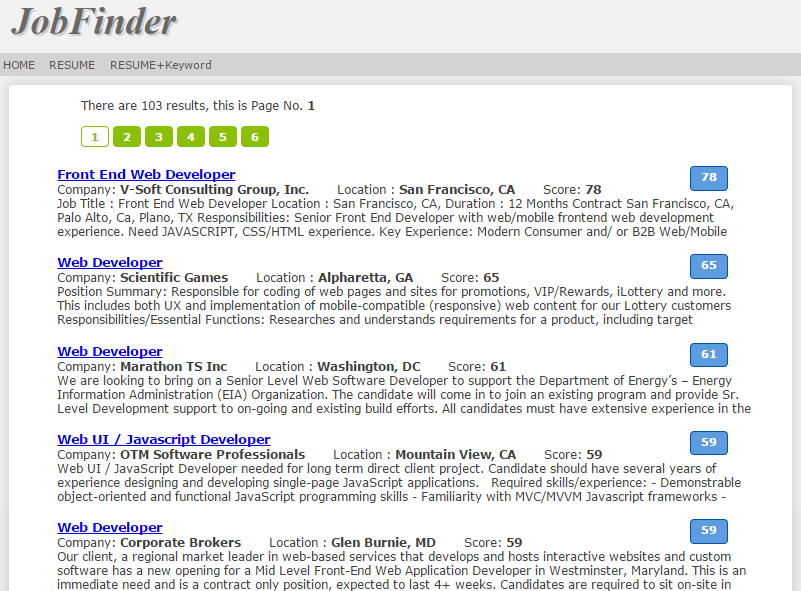
\includegraphics[scale=0.5]{images/match_resume.png}
%  \caption{Jobs returned by the system}
%  \label{fig:result}
%\end{figure}

\subsection{System Architecture Overview}
%\begin{enumerate}
%    \item The Web Crawler can access and download all new IT job opening web pages from indeed.com everyday.
%    \item The Job Parser can parse the job opening web pages, extract the information and create the job models.
%    \item The Resume Parser is much like the Job Parser; it parses the r\'esum\'es and creates the r\'esum\'e models.
%    \item All the job descriptions and job models are stored in the database.
%    \item When a user searches  the jobs with their r\'esum\'e, the Ontology Matcher calculates the similarity values of jobs in the database and returns the jobs ranked by their similarity values.
%\end{enumerate}
In this section, we provide an overview of the main components of the Resumatcher system. As illustrated in figure \ref{fig:arch}, the Resumatcher system comprises of the following main components: Job Data Processor, Search Interface, and the Resume Matcher.
\begin{figure}[htbp]
  \centering
  \includegraphics[scale=0.7]{images/arch_v2_folami.png}
  \caption{System Architecture}
  \label{fig:arch}
\end{figure}

\subsubsection{Jobs Data Processor}
\noindent The Jobs Data Processor component executes a daily batch job, which processes all new job listings posted on the web. It consists of the following modules:
\begin{enumerate}
\item Web Crawler: This component systematically browses job websites to help create an index of new job posts. The job crawler downloads web pages and intelligently extracts data specific to job posting (this filters and excludes all non-job related content such as advertising).

\item{Jobs Model Builder}: The Jobs Model builder parses and processes sentences contained in a job listing to extract job related information (such as location, required skills, required experience etc.). Content extracted from the job listing is further processed using a feature extraction algorithm to create a job model described by four features: a job title, major, academic degree, and required skills. The output of the Model Object builder is a job object which consists of a job description (content displayable to end user) and a job model, which consists of features as described above.

\end{enumerate}

\subsubsection{Search Interface}
\noindent The resume query interface provides a frontend interactive interface through which the prospective job seeker submits a resume and subsequently reviews relevant search results. The Search Interface consists of the following modules:
\begin{enumerate}
\item Query input module: This component allows the user to upload a resume document as the primary search parameter for a job search. This interface accepts resumes in Microsoft Word, PDF, and plain text format.

\item Resume Model Builder: The Resume Model Builder in the Search Interface processes content in a resume document to extract candidate related information. This includes such data related to academic or professional training and education, and skills. This data is then used to build a resume model object, which is used as the primary query item in the Resume Matcher component.

\end{enumerate}

\subsubsection{Resume Matcher}
\noindent This is the core component of the resumatcher system. The Resume Matcher receives as input, a resume object from the Query Interface, and queries the job database using a novel similarity method to retrieve the most relevant jobs. The similarity between a resume object and a job object is calculated as a weighted sum of the computed features. This proceedure is described in greater detail in section \ref{similarity}. A list of jobs are returned and displayed to the user in sorted order of similarity to the resume object via the Search Interface.


\section{Information Extraction}
\subsection{Information Extraction Overview}
In this section, we describe procedures used to extract job related content from job posting websites. Content from Internet job postings and uploaded resume content undergo a similar procedure which is comprised of six steps: preprocessing, semantic labeling, and pattern matching. These steps are illustrated in figure~\ref{fig:Pipeline}.

%HTML parsing, segmentation, preprocessing, string tokenization, semantic labeling and pattern matching. These steps are illustrated in figure~\ref{fig:Pipeline}.

%The information extraction framework for the Resumatcher system uses six stages in order to extract the information from job descriptions: HTML parsing, segmentation, preprocessing, tokenizing, labeling and pattern matching, which is shown in Figure~\ref{fig:Pipeline}.

\begin{figure}[htbp]
  \centering
  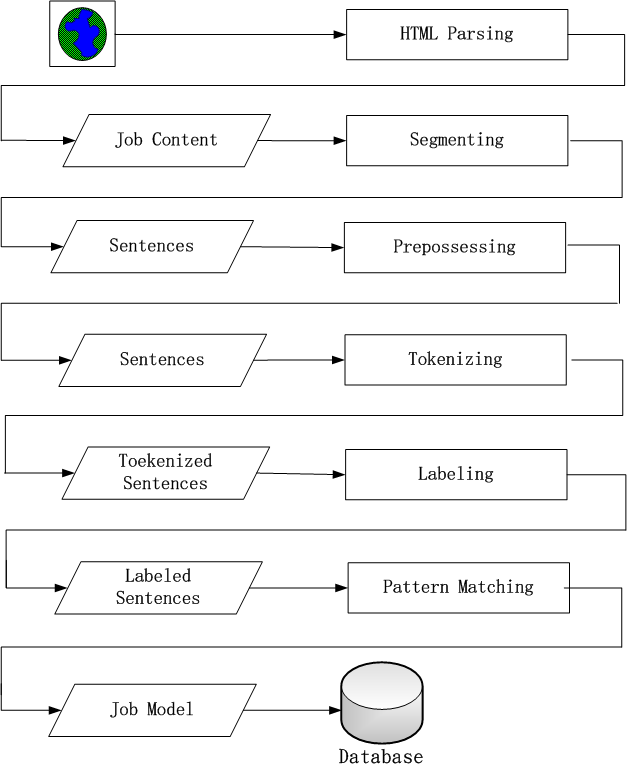
\includegraphics[scale=0.6]{images/pipeline2.png}
  \caption{Job Description Process Pipeline}
  \label{fig:Pipeline}
\end{figure}

\subsection{Preprocessing}
The preprocessing stage involves parsing and tokenization. Content from job postings or uploaded resumes are parsed to extract related attributes in the form of paragraphs and sentences. Attributes such as job title, job location, company, and job description are extracted from job postings, while professional skills, education, and experience are extracted from uploaded resumes. In the next stage, characters such as '/' and '-', which do not convey any meaningful information  are replaced with white spaces prior to tokenizing. Sentences are then tokenized into arrays of tokens using NLTK~\cite{bird2006nltk}.


%The \textbf{HTML Parsing} will parse the web pages that contain job descriptions, which are obtained from web crawler. The parser uses HTML tag template to extract attributes of the jobs, like job title, location, company name, content and so on. A job will be saved as a record with these attributes in the database. In the record, the content field contains the text part of the job description, which will be processed in later stages. In the \textbf{segmentation stage}, the content field of the job description is be separated into paragraphs according HTML tags. In the \textbf{preprocessing stage}, characters in the sentences are converted to ASCII characters, unreadable characters will be deleted, and some punctuation will be replaced by spaces (e.g. / and -). In the \textbf{tokenizing stage}, the sentences will be tokenized into arrays of tokens by NLTK~\cite{bird2006nltk}. In the \textbf{labeling stage}, the sentences will be given two layers of labels by a dictionary matching approach, which will be described in semantic labeling part. In the \textbf{pattern matching} stage, the FST library is used to matching the labels of the labeled sentences. If a layered sentence match any pre-defined pattern, the information will be extracted and added to the job model. After every sentence of a job description has be processed, a job model will be created and saved in the database.

%The IE framework will be introduced by example of processing the job descriptions. We use rule based method to extract the information from r\'esum\'es and job descriptions. To achieve this, we proposed  a Finite-State Transducer(FST) based pattern matching library.



\subsection{Semantic Labeling}

Natural Language Processing (NLP) poses a unique challenge in that the relationship between word and meaning is very often a many-to-many relationship, that is a single word can be used to express several concepts and vice versa. For example, the expression \textit{Bachelors degree} can be expressed several ways in a job description including \textit{B.S.} , \textit{BS}, \textit{4-year degree}, and so on. This challenge is further illustrated in Table \ref{tab:multispelling}, which provides a list of words that can be disambiguated to mean a semantic value of ``Bachelors degree''.


\begin{table}[ht]
\caption{Degree Words and Their Variants} % title of Table
\centering % used for centering table
\begin{tabular}{   l | l | l | l | l | l | l   }
 \hline\hline
 Word &  \multicolumn{6}{c}{Variants }  \\
\hline
 Baccalaureate &  bachelors  & bachelor & B.S.    &  B.A.  & BA/BS    &  Undergraduate  \\
%\hline
 Masters       &  M.S.       & M.E.     & Meng    &  MBA   & MSc      &  MS \\
%\hline
 Doctorate     &  PhD        & Ph.D.    & Doctor  &  Ph.D  &          &    \\
\hline
\end{tabular}
\label{tab:multispelling} % is used to refer this table in the text\section{Pipeline of Information Extraction}
\end{table}

Using the tokens generated from job or resume documents will result in a significant amount of overlap. Further, encoding this information in a finite state transducer (FST) will result in higher space complexity. To overcome this problem, we implement a pattern matching library which supports regular expressions over tokens. This method of semantic labeling maps multiple tokens to a unique label or hyponym. Each hyponym is subsequently mapped to a hypernym. Applying this process to the inputs in Table~\ref{tab:multispelling}, results in more simple semantic labelling map illustrated in Table~\ref{tab:semanticlabeling}.


%To add labels to a sentence, we use token pattern matching library which support a regular expression over tokens. If we use all the expressions of a semantic value to create a pattern, the pattern will be very large, and there are too many states in the FST. For example, if we use some words in Table~\ref{tab:multispelling} to create the pattern of semantic value ``bachelor's degree'', the pattern will like below:
%$$ (~Baccalaureate~\mid~bachelors~\mid~bachelor~~\mid~B.S~\mid~BS~\mid~BA~)~~degree $$
%If all words in Table~\ref{tab:multispelling} are added to the pattern, the FST will have too many edges, and the matching process will be very slow because of the problem of combinatorial explosion.

%To resolve this problem, we proposed an approach to use the patterns to match the \textit{labels} of the tokens, not the the original text. In the system, we don't care what words the sentences really use, but want to extract the semantic value of the tokens which match the pattern. The details of the approach is described below.

%At first, we created two dictionaries, which are used to label the tokens. In the first dictionary, the keys are the tokens, like words in Table~\ref{tab:multispelling}, and the values are the symbols for semantic values, like ``BS-LEVEL'' for ``bachelor's degree'', or ``MS-LEVEL'' for ``master's degree''. The values of the the second dictionary are the ontology hypernym of their keys, like keys ``BS-LEVEL'' and  ``MS-LEVEL'' both have value ``DE-LEVEL'', which means that bachelor's degree and master's degree are both one kind of degree level. We show the dictionaries for degree information in Table~\ref{tab:semanticlabeling}.

\begin{table}[ht]
\caption{Semantic Labeling } % title of Table
\centering % used for centering table
\small
\begin{tabular}{  l | l | c }
 \hline\hline
 Input Token & Hyponym & Hypernym\\
 \hline
   bachelors  &     &\\
 %\cline{1-1}
   bachelor   & \multirow{4}{*} ~BS-LEVEL    &\\
 %\cline{1-1}
   B.S.       &     &\\
 %\cline{1-1}
   Baccalaureate    &     &\\
 \cline{1-2}
   Master     &     &   \multirow{10}{*} ~DE-LEVEL\\
 %\cline{1-1}
   MS         &  \multirow{3}{*} ~MS-LEVEL   &\\
 %\cline{1-1}
   M.S.       &     &\\
 \cline{1-2}
   PhD        &        &\\
 %\cline{1-1}
 Ph.D         &  \multirow{3}{*} ~PHD-LEVEL   &\\
 %\cline{1-1}
  Doctorate   &     &\\
 \hline

\end{tabular}
\label{tab:semanticlabeling} % is used to refer this table in the text\section{Pipeline of Information Extraction}
\end{table}

This method of structured hierarchical mapping is achieved by implementing a dictionary mapping tokens to hyponyms, and hyponyms to hypernyms. Table~\ref{tab:labeldsent} shows the application of this method to a sample sentence from a job description.

%With the two dictionaries, we can label the tokens with two layers. Table~\ref{tab:labeldsent} shows how the sentence ``Bachelors  degree  in computer science or information systems.'' is labeled.

\begin{table}[ht]
\caption{Labeled sentence } % title of Table
\centering % used for centering table
\small
\begin{tabular}{  l | l | l | l | l | l | l }
 \hline\hline
 Semantic Layer & \multicolumn{6}{c}{Expression}\\
 \hline
 Token & bachelors   & degree & in & computer science & or & information systems\\
 Hyponym &  BS-LEVEL   & DEGREE & IN & MAJOR-CS         & OR & MAJOR-INFO\\
 Hypernym & DE-LEVEL   & DEGREE & IN & MAJOR            & OR & MAJOR  \\
 \hline
\end{tabular}
\label{tab:labeldsent} % is used to refer this table in the text\section{Pipeline of Information Extraction}
\end{table}

The output pattern ``DE-LEVEL DEGREE  IN   MAJOR  OR  MAJOR" provides a condensed representation of the input token string, thereby reducing the spatial complexity in encoding a large number  unique patterns represented in our FST, and a faster running time in the pattern matching process. % YOU NEED TO SHOW SOME DATA capturing this improvement.

%The pattern ``DE-LEVEL DEGREE  IN   MAJOR  OR  MAJOR ''  can match the sentence above, and the output of the matching process is ``BS-LEVEL'' for bachelor's degree, ``MAJOR-CS'' and ``MAJOR-INFO'' for two majors mentioned in sentence. In our system, most patterns match the labels in second layer. With this approach, the size of the FST for the pattern will be minimized, so speed of matching process can be improved.




\subsection{Pattern Matching Library}

Finite-state machines have been used in various domains of natural language processing especially in computational linguistics. Linguistically, in using finite automata we can easily describe the relevant information encountered in a language. This results in a compact representation of lexical rules, or idioms and clich��es \cite{gross1989use}. From a computational point of view however, finite-state machines serve to improve time and space efficiency

A finite state transducer (FST) is a finite state machine which, given an input string, is able to generate a unique output string. For the Resumatcher system, we developed a flexible, lightweight FST framework, capable of processing regular expression matching over labeled tokens. Our FST library supports regular expression, operator and object-oriented expressions as input. Providing support for operator and object-oriented expression allows for greater flexibility in customizing the library for other domains.

%After studying currrent FST based tools, we found most of them to be powerful and complex, but not very flexible. One reason is that developers need to learn some Domain specific Languages (DSLs) like CPSL. The other reason is the extra effort and time required to integrate the pattern matching tool into the system. So here we proposed a more flexible and lightweight FST framework, which can do regular expression matching over labeled tokens. To convert a regular expression over token to a FST we need two steps: The first is parsing the expression to a tree of matchers, the second is transfer the tree of matchers to the FST. We will introduce these two steps in next.

%In our library, a ``matcher'' could be a token to be matched, or a composition of other matchers. Our library supports syntax used in traditional regular expressions over strings. We list the syntax that the library supports in Table~\ref{tab:matchers}. The first column is the names of the matchers, the second column is the explanation of the function of the matchers, and third column is the their counterpart syntaxes of traditional regular expression. The RegexMatcher in our library is constructed with a regular expression, and the matcher matches any string that matches the regular expression in the matcher.

\begin{table}[ht]
\caption{Matchers of our Library } % title of Table
\centering % used for centering table
\begin{tabular}{   l | l | l   }
 \hline\hline

 Matcher Type      &  Description                              & Regex Counterpart   \\
 \hline
 UnitMatcher       &  token is matches the it                  & regular characters       \\
 %\hline
 SequenceMatcher   &  A list of Matcher                        & sequence of characters       \\
 % \hline
 QuestionMatcher   &  One or more of the preceding token       & ?       \\
 % \hline
 StarMatcher       &  Zero or more of the preceding token      & *       \\
 % \hline
 PlusMatcher       &  Zero or one of the preceding token       & +       \\
 % \hline
 DotMatcher        &  Any token                                & .      \\
 % \hline
 RegexMatcher      &  Any token matches the regular expression               &  N/A      \\
  \hline
\end{tabular}
\label{tab:matchers} % is used to refer this table in the text\section{Pipeline of Information Extraction}
\end{table}


The framework supports three styles of creating patterns: regular expression style, operator style and object-oriented style. The second and third styles are flexible because developers can create their own matcher class to extend the feature of the library. We use examples to show how the three styles work. The most common style is defining pattern expression in a string, which is much like traditional regular expression.

%\begin{framed}
%\small
%\noindent
%The pattern is:  DE-LEVEL DEGREE ( IN  $\vert$  OF ) DT? MAJOR \\
%The code is: \\
%seqMatcher =parser.parse("DE-LEVEL DEGREE ( IN  $\vert$  OF ) DT? MAJOR")

%\end{framed}

%The second style is using algebraic operators to connect matchers, which can help developer reuse previous patterns when the new patterns include old ones. It is shown in follows:
%\begin{framed}
%\small
%\noindent
%The pattern is:  "DE-LEVEL DEGREE (IN $\vert$ OF) MAJOR" \\
%The code is: \\
%seqMatcher =  UnitMatcher("DE-LEVEL") +  UnitMatcher("DEGREE") + \\
%\hspace{3cm} ( UnitMatcher("IN") $\vert$ UnitMatcher("OF" ) ) + UnitMatcher("MAJOR")

%\end{framed}

%We also could create a complex matcher in object-oriented programming style.

%\begin{framed}
%\small
%\noindent
%The pattern is:  "DE-LEVEL DEGREE (IN $\vert$ OF) MAJOR" \\
%The code is: \\
%matcher1 = UnitMatcher("DE-LEVEL") \\
%matcher2 = UnitMatcher("DEGREE")  \\
%matcher3 = UnitMatcher("IN")   \\
%matcher4 = UnitMatcher("OF")   \\
%matcher5 = UnitMatcher("MAJOR")  \\
%matcher6 = AlternateMatcher([matcher3,matcher4])   \\
%seqMatcher = SeqMatcher([matcher1, matcher2, matcher6, matcher5])
%\end{framed}


%You need to explain this part to me. It does not make any sense and so i don't understand why it is here.

%\subsection{Patterns for Matching }

%As we explained in section B, we mentioned matching tokens in the second layer to patterns we defined. To match the labels in sentences to our patterns, we proposed a library that support matching pattern over tokens. The difference between this library and traditional regular expression is that the basic unit to be matched is token, not character. Some patterns used to match degree phrases are in Table~\ref{tab:patterns}. The patterns looks like regular expression, but they use tokens as the basic units.

%\begin{table}[ht]
%\small
%\caption{Patterns to match degree sentences} % title of Table
%\centering % used for centering table
%\begin{tabular}{  | l  |  }
% \hline
% DE-LEVEL,  DE-LEVEL, OR  DE-LEVEL DEGREE   \\
% DE-LEVEL DEGREE ( IN  $\vert$  OF ) DT MAJOR   \\
% MAJOR-DEGREE  ,  MAJOR-DEGREE OR MAJOR \\
% DE-LEVEL (, DE-LEVEL)* (OR DE-LEVEL)? BE? PERFER-VBD   \\
% \hline
%\end{tabular}
%\label{tab:patterns} % is used to refer this table in the text\section{Pipeline of Information Extraction}
%\end{table}


\section{Skills Similarity Measures for Resumes and Jobs}
In this section, we describe a methodology for extracting skills from both job postings and resume submissions to build a domain specific skills library. Using this library, we develop an ontology of skills as a framework for relationship between skills. From the constraints provided by this framework, we describe how to quantify the similarity between skills.

\subsection{Domain Specific Skills Library}
One major challenge in the job search process is the ability to match required job skills with a candidate possessing such skills. The first step in the process is to understand the skills required for the job. Using sentences extracted from actual job descriptions in Table~\ref{tab:skillrequirement}, we observed the following characteristics:
\begin{enumerate}
\item Job postings provide information on required skills explicitly
\item Required skills in job postings are enumerated in one or more sentences
\item A majority of job postings require more than a single skill
\end{enumerate}

\noindent To take advantage of these constraints, we have developed a template matching machine learning algorithm to automatically learn what job skills are and extract them from both job postings and resumes. First we construct a skills dictionary using a few known skills. This skills dictionary is updated iteratively using a training set of job descriptions. For each job description, we extract one or more skills sentences. A skill sentence is any sentence within a job description identified as having at least two known skills (known skills are those present in the skills database). The skill-sentence is tokenized and processed to remove stop words. This process results in a collection of tokens, some of which are known skills. Each unknown token is validated to be an actual skill by cross-referencing with \href{http://dbpedia.org/page/XSL}{\textit{DBpedia}}. \href{http://dbpedia.org/page/XSL}{\textit{DBpedia}} is a crowd-sourced community effort to extract structured information from \textit{Wikipedia} and make this information available on the Web. DBpedia allows you to ask sophisticated queries against \textit{Wikipedia}. After successful validation, each new skill is added to the skills dictionary thereby expanding the size and effectiveness of discovering new skills with each new training iteration.


%The primary goal of the job search process is to match the right job to the right candidate. This requires matching skills indicated in the job posting with a candidate who's resume contains the required skills. To achieve this goal, we a template matching algorithm for automatically extracting a candidate's job skills from their provided resume.

%\subsection{Construct Ontology for Skills}

%From observation, we find that sentences containing skill requirements in a job description lists two or more skills. An example of this is shown in Table ~\ref{tab:skillrequirement}. Based on this observation, we developed a clustered template matching algorithm that identifies skills based on the k-nearest neighbor words as listed in the job description.

%First, we manually collect about fifty terms from job descriptions, and add them to the term list. Then we use our pattern match library to find the sentences that matching the pattern in Table \ref{tab:termpatterns} from a set of job descriptions. An example of a sentence which matches the pattern is shown in Table \ref{tab:termspattern}. We extract the tokens which match the star symbol from the sentences; these tokens have high probability to be technical terms. Then we could check the tokens in Dbpedia to see whether they are under the categories like software, programming language or any other technical related ones. If they are, we could classify them as terms, and add them to the terms list. After scanning all the sentences in the job description set, the term list will be larger, and we can use the larger term list to start a new iteration of scanning. This process stops when the number of found new terms is below a threshold. The process is shown Figure~\ref{fig:gen_onto}.

\begin{table}[ht]
\caption{Skill requirements as listed in job description} % title of Table
\centering % used for centering table
\begin{tabular}{ l | l }
 \hline\hline
    1 & A high-level language such as Java, Ruby or Python; we use Java and Groovy extensively \\
    2 & HTML5/CSS3/JavaScript, web standards, jQuery or frameworks like AngularJS would be great\\
    3 & HTML CSS and Javascript a must\\
    4 & Experience with AJAX, XML, XSL, XSLT, CSS, JavaScript, JQuery, HTML and Web Services   \\
 \hline
\end{tabular}
\label{tab:skillrequirement} % is used to refer this table in the text
\end{table}


%\begin{table}[ht]
%\caption{Patterns to extract terms} % title of Table
%\centering % used for centering table
%\begin{tabular}{   | p{8cm} |  }
% \hline
%     term   , * , *,  term  \\  \hline
%     term  , * , *, and  term   \\
% \hline
%\end{tabular}
%\label{tab:termpatterns} % is used to refer this table in the text
%\end{table}

\begin{comment}

\begin{table}[ht]
\caption{An example sentence matches the pattern} % title of Table
\centering % used for centering table
\begin{tabular}{   | c | c | c | c |c | c |c | c |c | c |c | c |c | c |  }
 \hline
     Experience & with & TERM & , & *   & , & *   &, & TERM &, & and & *  \\
 \hline
     Experience & with & AJAX & , & XML & , & XSL &, & XSLT &, & and & CSS  \\
 \hline
\end{tabular}
\label{tab:termspattern} % is used to refer this table in the text
\end{table}
\end{comment}

%For example, we extract the token  ''XSL'', which currently is not in the terms list. We check the word on DBpedia by accessing the URL:http://dbpedia.org/page/XSL. If we can get the XML formatted description of XSL, and any element in ``dcterms:subject'' section has the value which is a technical category,  like ``Programming languages'', ``Markup languages'' and so on, we can indicate that the word is a technical term, and add it to the term list.

%\begin{figure}[htbp]
%  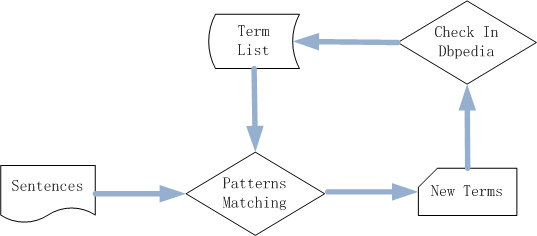
\includegraphics[scale=0.6]{images/genonto.png}
%  \caption{Procedure of Finding Technical Terms}
%  \label{fig:gen_onto}
%\end{figure}


%We observed that simple keyword matching is not a good similarity measure, because job descriptions and r\'esum\'es both contain richer and more complex words that cannot be described simply by keywords. In these documents, some concepts can be written in different ways, and other concepts can have close relationships. For example, Table~\ref{tab:resume_jd} shows portions of a r\'esum\'e and a job description:

%If just looking at the text, we can find that the r\'esum\'e has very few common words with the job description. But from the view of an experienced engineer, the candidate is closely matches the job: the two relational databases Oracle and Mysql are very similar, OOA/OOD is the same meaning of many years of Java and C++ experience, and Tomcat and JBOSS are both Java web applications servers. If we use keyword matching, the system does not provide a strong matching result in very common cases such as this. So we need a better approach to calculate the similarity between different technical concepts.


\subsection{Skills Similarity Measures for Resumes and Jobs}

Current systems base search results on keyword matching. While this method provides plausible results, it does not use linguistic properties specific to the domain. When we consider text used in job descriptions and resumes to describe job requirements and personal qualifications respectively, we find hierarchical relationships between skills and qualifications. Secondly, a significant amount of ambiguity exists between domain specific words and their respective interpretation. This ambiguity is illustrated in Figure~
%Add figure reference here
, which shows sentences extracted from resumes and job descriptions.



We observed that simple keyword matching is not a good similarity measure, because job descriptions and r\'esum\'es both contain richer and more complex words that cannot be described simply by keywords. In these documents, some concepts can be written in different ways, and other concepts can have close relationships. For example, Table~\ref{tab:resume_jd} shows portions of a r\'esum\'e and a job description:

\begin{table}[ht]
\caption{An example of Job Description and R\'esum\'e} % title of Table
\centering % used for centering table
\begin{tabular}{   | l |    }
 \hline
   \textbf{ Job Description}  \\
 \hline
3+ years development experience in Java and OOA/OOD ~~~~~~~~~~ \\
2+ years in Java, JSP, J2EE, SQL, VXML, Web-services environment \\
2+ years XML, XSL, XML Beans \\
Strong MS SQL Server, MySql \\
Familiarity with Apache, Tomcat, JBoss, Struts and Web Services \\
Familiarity with test driven development \\
Experience working in Agile methodology  \\
 \hline
    \textbf{R\'esum\'e }\\
 \hline
Technical Skills: \\

Languages Java, C++, HTML, HTML5, XML, PL/SQL \\
J2EE Technologies Java J2EE, Servlets, JSP, Struts, Java web application servers \\
Version Control CVS, Bugzilla, SVN, PVCS: Ant, Maven  \\
Experience in Oracle 11g, PostgreSQL \\
NoSQL: MongoDB, HBase, Cassandra \\


  \hline
\end{tabular}
\label{tab:resume_jd} % is used to refer this table in the text
\end{table}



From the resume illustrated in the Table~\ref{tab:resume_jd}~
% add reference to resume figure
we observe that a keyword search will incorrectly find that this resume is not a suitable match for the job description illustrated in Figure~
% add reference to job figure
. However, we observe intuitively that relationships exists between some of the skills listed in the candidate resume and the requirements from the job description. For example, \textit{experience in Oracle database} demonstrates a level of competence for a job that requires \textit{Mysql}, and \textit{MS-SQL} skills. Similarly, knowledge and experience with object oriented programming and design viz \textit{OOA/OOD}, is evidenced with \textit{Java} and \textit{C++} programming experience. In the same manner, \textit{Tomcat} and \textit{JBOSS} are both considered \textit{Java web application servers}. To overcome these deficiencies, we propose a novel ontology based similarity measure, details of which are presented in the following sections.

%If just looking at the text, we can find that the r\'esum\'e has very few common words with the job description. But from the view of an experienced engineer, the candidate is closely matches the job: the two relational databases Oracle and Mysql are very similar, OOA/OOD is the same meaning of many years of Java and C++ experience, and Tomcat and JBOSS are both Java web applications servers. If we use keyword matching, the system does not provide a strong matching result in very common cases such as this. So we need a better approach to calculate the similarity between different technical concepts.
\subsection{Constructing an Ontology of Skills}
To incorporate the observed interrelationships that exist between skills and experience within the context of job search, we have developed a domain specific ontology of skills. An \textit{ontology} provides a formal definition of objects, properties, and interrelationships between objects for a the given domain. Thus creating a taxonomy, which compartmentalizes variables needed for computing similarities between skills, thereby establishing formal relationships between them. Taking advantage of the taxonomy provided through \href{http://dbpedia.org/page/XSL}{\textit{DBpedia}}, we combine the this structure with a novel similarity measure to establish a formal relationship between skills.

%\begin{comment}
\begin{figure}[htbp]
\centering
  \includegraphics[scale=0.5]{images/onto_2.png}
  \caption{Programming Language Ontology}
  \label{fig:ontology_pro}
\end{figure}
%\end{comment}

\subsection{Computing Similarity Measure}

The Skills ontology framework provides a real-world constraint on relationships between skills. Within this framework, a skill $a$ is said to be similar to another skill $b$ if at least one of the following conditions are met:
\begin{enumerate}
\item{Skill A is a hypernym of skill B}
\item{Skill A is a hyponym of skill B}
\item{Skill A and Skill B share the same hypernym}
\end{enumerate}

Given two skills, $a$ and $b$, both having the same direct hypernym or one is the hypernym of the other, we define similarity $sim(a,b)$ between $a$ and $b$ as:

\begin{equation}
\label{eq:simskills}
sim(a,b) = \frac{jaccard(A,B)}{\log_2\Big\{\frac{1}{N_{a \cap b}}\mathlarger{\sum}\limits^{N_{a \cap b}}_{k=1} \argmin\limits_{i,j} \left|\left| d^k_{a_i} - d^k_{b_j} \right|\right|\Big\}}
\end{equation}

\noindent Where $jaccard(A,B)$ is defined as: $jaccard(A,B) = \frac{N_{a \cap b}}{N_{a \cup b}}$.\newline
$N_{a \cap b}$ is the number of documents $d_{a \cap b}$ where skills $a$ and $b$ are both present.\newline
$N_{a \cup b}$ is the number of documents $d_{a \cup b}$ where either skill $a$ or skill $b$ is present.\newline
$d^k_{a_i}$ is the term index for the $i^{th}$ occurrence of skill $a$ in the $k^{th}$ $d_{a \cap b}$ document.\newline
$d^k_{b_j}$ is the term index for the $j^{th}$ occurrence of skill $b$ in the $k^{th}$ $d_{a \cap b}$ document.\newline


%the Jaccard coefficient, as a measure of the similarity between sets A and B, and is defined as the size of the intersection divided by the size of the union of the sample sets
%Once we establish a relationship between skills, the similarity between two skills is quantified using eq~\ref{eq:simskills}:
%A majority of job descriptions list multiple skills required for the job position. From observation, we find that related skills always exist in the job description simultaneously, and the positions of them are always close, e.g. HTML and CSS are always required together, and appear in the same sentence. We can see from the Table~\ref{tab:skillrequirement}, the closely related concepts are always have short distance. Based on such observation, we give a new statistical-based ontology similarity measure.

%Where \frac{  N_{a \cap b} numerator is the ratio of the number of documents in which the two terms exist together $(N_{a \cap b})$ and the number of documents have a least one of them $(N_{a \cup b})$. The denominator is the average $\log$ value of minimum distance $mindis(doc,a,b)$ of the two terms in documents that have them both.

%We set the restriction on the position of the two concepts in the ontology, because the position of the concepts in the ontology are based on their technical similarity to others. Similar techniques will be assigned into the same category, so they should share the same hypernym, and one could be an alternative to the other. For example, we put EJB and Hibernate in the same category, because they are both J2EE persistence layer technologies, and both have the O/R mapping concept. If the applicant is familiar one of them, they can master the other very quickly. Another example is Grail and Django, they are both web frameworks and share same web design philosophies, but one of them is designed for Java web application and the other is created for Python web application. If a developer has some some experience with one of them, he/she still need to spend a lot of time to learn the other to overcome the gap between programming languages.


\section{Document Model Similarity}
\label{similarity}

%include a sample document illustrating fields of a resume object and a document object.
The document model describes the model of a job description document (\textit{job objects}) or a resume document (\textit{resume object}). Both objects are constituent of similar fields: job title, college major, academic degree, and technical skills. Once we obtain an object representation of both job description (\textit{job objects}) and resume documents (\textit{resume objects}), we are able to compare both objects by computing a weighted similarity measure. Formally, we define the similarity between a \textit{job objects} $d_j$ and a \textit{resume objects} $d_r$ as the weighted sum of the distance between corresponding fields in both documents.
\begin{equation}
sim(d^i_j,d^i_r) = \sum_{i=1}^{n} \mathlarger{\lambda}_i(d^i_j,d^i_r) \times \omega_i
\end{equation}

Where $\lambda_i(d_{j_i},d_{r_i})$ is a distance function for the $i^{th}$ field between both objects, and $\omega_i$ is an empirically determined weight term for the $i^{th}$ field. In the following sections, we provide a detailed description of $\lambda$ for each field.

%The value of $sim(r, j)$ is the summation of similarity values of different fields times their corresponding weights. $simfun_i(r_i,j_i)$ is the similarity function of the $ith$ field of the model. In our system, the r\'esum\'e model and job model both have four fields: job title, major, academic degree and skills. The similarity value between a r\'esum\'e model and job model is the sum of the productions of similarity values of all the fields pairs and their weights. We will introduce how to calculate the similarity value for each field in this section.

\subsection{College Major Similarity}

%What list of majors are you referring to? Where is this list mentioned in the paper?
In the simplest case, if the majors in the r\'esum\'e model and job model are the same, the similarity value is 1. If they are different, we can check whether the major in the r\'esum\'e model is in the list of related majors for the major listed in the job model. If this is the case, the similarity value is 0.5; otherwise the similarity value is 0. The computation for major similarity $\lambda_{m}$ is shown below:
\begin{equation}
\mathlarger{\lambda}_{m}(m_j,m_r) =
\begin{Bmatrix}
1, & m_j = m_r \\
0.5, & m_j \in hypernym(m_r) \| m_j \in hyponym(m_r) \| hypernym(m_j) = hypernym(m_r)\\
0, & otherwise
\end{Bmatrix}
\end{equation}
Where $m_j$ and $m_r$ represent the college major listed in the job description and the resume respectively.

\subsection{Academic Degree Similarity}

Using the five major types of academic degrees (High School Diploma, Associates, Bachelors, Masters, and Doctoral degrees), we assign each degree to a unique integer value between 1 and 5. In this method, more advanced degrees are assigned a higher numeric value (e.g. A doctoral degree is assigned a value of 5, while a High School diploma is assigned a value of 1). Based on these numerical values, we calculate the academic degree similarity $\lambda_{d}$ using the following equation:

%If the degree value in the r\'esum\'e model is less than that in the job model, which means that the job seeker's education background cannot satisfy the requirement of the job, the similarity value in this case is 0. If the degree value in the r\'esum\'e model is equal to the job model and no more than 2 above, the similarity value is 1. In some cases, the degree value in the r\'esum\'e model is greater than that of the job model, and the difference is greater than 2, which means that the job seeker's degree is much higher than the requirement of the job. The situation is also a kind of relative matching, so the similarity value here is 0.5. The equation is shown below:

\begin{equation}
\mathlarger{\lambda_{d}}(d_j,d_r) =
\begin{Bmatrix}
0,   & d_j < d_r \\
1,   & \|d_j - d_r\| \leqslant 2  \\
0.5, & \|d_j - d_r\| > 2
\end{Bmatrix}
\end{equation}
Where $d_j$ and $d_r$ represent the academic degree listed in the job description and the resume respectively.

\subsection{Job Title Similarity}

The title of a job description contains information that can be separated into unique segments including functional role (developer, tester, architect), hierarchical level (junior, senior), platform (web, mobile, network, cloud), programming language, and domain. There are typically multiple titles in a single resume, reflecting a job candidate's prior experience. This results in a one to many comparison between job object title and resume object titles. We determine the similarity between the job title and the resume titles by calculating the distance between all resume titles and selecting the title with the highest numerical value. We calculate the similarity between job titles using the following equation:

\begin{equation}
\mathlarger{\lambda_{t}}(t_j,t_r) = \argmax\limits_k\Big\{\frac{1}{n} \sum\limits^n_{i=1} sim_k(t_{j_i},t_{r_i}) \Big\}
\end{equation}
Where $sim_k(t_{j_i},t_{r_i}) =
\begin{Bmatrix}
1,   & t_{j_i}=t_{r_i} \\
0,   & otherwise
\end{Bmatrix}
$\\
$k$ is the number of unique job titles contained in a resume object,
$n$ is the number of unique segments within a resume job title,
$t_{r_i}$ and $t_{j_i}$ represent the $i^{th}$ term in the title of the resume object and job object respectively.


%A job title can be parsed into some sub fields: job role, level, platform, programming language.  The value of job roles includes: developer, manager, administrator and so on. There are levels values in such roles: such as junior, senior and architect. The platforms: web, mobile and cloud are used by the very roles.  The similarity value between two titles is the sum of all the similarity values of these fields. The similarity value of each subfield ranges from 0 to 1, and we also normalized the similarity summation value to 1 by dividing the number of sub fields. If the job seeker has some working experience, there may be some job titles in their r\'esum\'e.  When calculating the similarity value between a r\'esum\'e model and a job model, the system calculates the similarity values of the title of job model to all the titles in the r\'esum\'e model and returns the maximum one.

\subsection{Technical Skills Similarity}

As described previously, we developed an ontology of skills with which we determine the similarity between skills. Using on this framework, we compute the similairty $\lambda_{s}$ between skills listed in job object $s_j$ and skills listed in resume object $s_r$ as follows:

%The job model usually has requirements of some skills, and the r\'esum\'e model lists the skills the job seeker has as well. The similarity value of skills field is the summation of all the similarity values of skills in the job model. For every skill in the job model, the similarity value is the maximum value it can get from the skills in the r\'esum\'e model. The equation is shown below:

\begin{equation}
\lambda_{s}(s_j,s_r ) = \frac{1}{n}\mathlarger{\sum}\limits^{n}_{i=1} \argmax\limits_{m} \Big\{sim(s_{j_n}, s_{r_m})\Big\}
\end{equation}

Where the similarity $sim(s_{j_n}, s_{r_m})$ between skills $s_{j_n}$ and $s_{r_m}$ is computed as defined in equation~\ref{eq:simskills}, $n$ is the number of skills listed in the job description, and $m$ is the number of skills listed in the resume.


\section{System Evaluation}
In this section, we describe the methodology used to evaluate major system components and the overall performance of the Resumatcher system.

\subsection{Information Extraction}
To evaluate the performance of the information extraction module, we measure the accuracy of sentence filters in identifying sentences whose content pertains to an applicant's college degree information.

In this experiment, we selected 100 sentences from existing job descriptions. The contents of each sentence defined candidate degree and college major requirements for a job posting. The values for "degree" and "major" were manually labelled. Content patterns were identified from each sentences to match and extract degree information. With 6 patterns, we obtain an accuracy of 94\% for predicting type of ``degree." We compare results from our method to results obtained using the conditional random fields (CRFs) model~\cite{lafferty2001conditional}, which is a state of art in machine learning model for sequence labeling.


\subsection{Ontology-Based Similarity}
To test the accuracy of similarity measures used by the Resumatcher system, we compare the ranking of the Resumatcher ontology-based similarity scores on 8 skills from a collection of 500 job descriptions with a pairwise similarity measure between skills provided by domain experts. Table~\ref{tab:dismatrix1} is a matrix of ontology-based similarity scores from the Resumatcher system and Table~\ref{tab:dismatrix2} %change this to correct table when added
is a matrix of averaged similarity scores provided by domain experts.
%in Table~\ref{tab:dismatrix2}. Higher values correspond to greater similarities, so the similarity between one skill and itself is 1. We selected one concept and ranked the other concepts by their similarity values to this concept. Human judges helped rank these concepts by assigning them "relevance scores" so that we can use NDCG to evaluate the effectiveness of our approach.
We use the $Normalized~Discounted~Cumulative~Gain ( NDCG )$ ~\cite{manning2008introduction} as a measure of ranking quality. NDCG is used in the field of information retrieval to measure effectiveness of web search engine algorithms or related applications. DCG measures the usefulness of a document by comparing its position in the result list against the graded relevance scale of documents returned in a result set.
% $$ NDCG = \frac {DCG}{IDCG} $$

%DCG is the measure of how documents are ranked according to their relevance scores, and IDCG is the DCG value that the documents are strictly sorted by their relevance values.
%$$DCG =  \sum_{i=1}^{p} \frac {2^{rel_i} - 1}{\log_2(i+1)} $$

\begin{table}
\centering
\caption{Pairwise ontology-based similarity measures}
\begin{tabular}{ c | c c c c c c c c }
 \hline
  \textbf{Skill}       & \textbf{Javascript} & \textbf{jQuery} &  \textbf{HTML}  &  \textbf{CSS}   &  \textbf{Java}  & \textbf{Python} &  \textbf{Ruby}  & \textbf{ JSP  }  \\  \hline
  \textbf{Javascript} &     1     %& 0.1981 & 0.2087 & 0.2439 & 0.0665 & 0.0189 & 0.023  & 0.0253   \\
  \\
    \textbf{jQuery}   &   0.1981   &   1    %& 0.0979 & 0.1328 & 0.0439 & 0.0142 & 0.0266 & 0.0232    \\
    \\
     \textbf{HTML}    &   0.2087   & 0.0979 &   1    %& 0.3569 & 0.0473 & 0.0175 & 0.023  & 0.0103   \\
     \\
     \textbf{CSS}     &   0.2439   & 0.1328 & 0.3569 &   1    %& 0.0537 & 0.0153 & 0.0181 & 0.015    \\
     \\
     \textbf{Java}    &   0.0665   & 0.0439 & 0.0473 & 0.0537 &   1    %& 0.0498 & 0.0287 & 0.075    \\
     \\
    \textbf{Python}   &   0.0189   & 0.0142 & 0.0175 & 0.0153 & 0.0498 &   1    %& 0.1333 & 0.0025   \\
    \\
     \textbf{Ruby}    &   0.023    & 0.0266 & 0.023  & 0.0181 & 0.0287 & 0.1333 &   1   %& 0.012    \\
     \\
     \textbf{JSP}     &   0.0253   & 0.0232 & 0.0103 & 0.015  & 0.075  & 0.0025 & 0.012  &   1      \\
 \hline
\end{tabular}
\label{tab:dismatrix1}
\end{table}


\subsection{Overall System Evaluation}
\subsubsection{Comparison with Alternative Retrieval Models}
We created a data set of 100 job descriptions, for a diverse set of jobs such as web developer, server back-end developer, mobile developer etc. Using 5 candidate r\'esum\'es, we queried the corpus of 100 jobs using the Resumatcher system to retrieve the top 20 jobs.  We used the average ranking provided by domain experts as ground-truth measure of relevance of each job description to a given r\'esum\'e.
To compare performance of the Resumatcher system with other retrieval methods, we use both Precision@K and NDCG. Precision@K measures the proportion of relevant documents in the first $k$ positions but disregards the individual position of each document.

%$$ P@k = \frac{1}{k} \sum^m_{i=1} l_i 1 \left(  r(i) \leq k  \right )  $$
%Where 1 is the indicator function: $1(A) = 1$ if A is true, 0 otherwise.

Using these two measures, we compare the performance of the Resumatcher system with three established retrieval models: Kullback-Leibler divergence algorithm~\cite{zhai2008statistical},  TF-IDF~\cite{manning2008introduction} and Okapi BM25~\cite{robertson1995okapi}.
Kullback-Leibler divergence provides a non-symmetric measure of the difference between two documents.
The term frequency-inverse document frequency ($tf-idf$), is a numerical statistic, which measures the importance of a word to a document within a collection and can be used as a model for comparing the similarity between documents.
Okapi BM25 is a bag-of-words retrieval model that ranks a set of documents based on the query terms appearing in each document.

\begin{comment}
The score of a document $D$ with respect to query $Q$ is given by:
\begin{equation}
    \begin{array}{rcl}
        s(D,Q) & = & -D( \theta_Q \parallel  \theta_D )\\
               & = &- \sum_{ \omega \in V } p (\omega \mid \theta_Q) \log \frac{ p (\omega \mid \theta_Q )}{p(\omega \mid \theta_D)} \\

    \end{array}
\end{equation}

In the equation $\theta_Q$ is the language model for a query, and  $\theta_D$ is the language model for a document.
\end{comment}

\begin{comment}
TF-IDF is a Vector Space Model, which calculates the similarity between the vectors of the query $q$ and the document $d$. In the equation, $tf$ is the term frequency, and $idf$ is the inverse document frequency. The TF-IDF weighting scheme assigned to term $t$ a weight in document $d$ given by:
$$ tf\text{-}idf_{t,d} = tf_{t,d} \times idf_{t} $$
The similarity between the query $q$ and the document $d$ given by:
$$ score(q,d) =  \sum_{t \in q }  tf\text{-}idf_{t,d} $$
\end{comment}

\begin{comment}
Given a query $q$, the BM25 score of a document $d$ is:

$$ score(q,d) = \sum_{ t \in q  }  idf_t \frac {tf_{t,d} \cdot(k_1 +1) }  {tf_{t,d} +k_1 \cdot ( 1-b + b\cdot \frac { \left | D \right |}{avgdl})}  $$

In the formula, $idf_t$ is IDF value of term $t$, $tf$ is the term frequency; $ |D|$ is the length of the document $D$; $avgdl$ is the average length of all the documents, and $k_1$ and $b$ are the free parameters.
\end{comment}


\subsubsection{Comparison with Keyword Search}
We compared the quality of search results between using the Resumatcher system and keyword-based search, which is generally used on job search websites. In this experiment, we used a skill listed in a given r\'esum\'e (e.g. ``Java'') as a query term on \url{www.indeed.com}. The first 100 results returned by \url{www.indeed.com} were stored and used as a jobs database. Using the same r\'esum\'e as query term, we used the Resumatcher system to retrieve the top 20 jobs from the created jobs database. Using Precition@k and DCG, we compare the top 20 keyword search results with the Resumatcher query results.


\section{EXPERIMENTAL RESULT}

\subsection{Information Extraction}
Table~\ref{tab:ieaccura} provides accuracy results of information extraction for three fields using the Resumatcher content matching method, and the conditional random fields (CRF) model.
\begin{table}[ht]
\caption{Information Extraction} % title of Table
\centering % used for centering table
\begin{tabular}{   c | c | c | c   }
 \hline
          \textbf{Field}   & \textbf{Unique Patterns} & \textbf{Resumatcher}  & \textbf{CRF}   \\
 \hline
          Degree  & 6           & 0.94       &  0.85  \\
 \hline
          Major   & 10          & 0.85       &  0.72  \\
 \hline

\end{tabular}
\label{tab:ieaccura} % is used to refer this table in the text
\end{table}



\subsection{Ontology-Based Similarity}

Table~\ref{tab:dismatrix1} gives the pairwise ontology-based similarity measures for 10 skills from a collection of 500 job descriptions. In %Table~\ref{tab:}
%add second table from judge rankings
, we show the averaged pairwise similarity scores from 10 domain experts on the same set o skills. %Table~\ref{tab:}
%add table of NDCG scores for all skills
shows the computed NDCG scores for each skill, which is shown is Table~\ref{tab:skillndcg}

\begin{table}
\centering
\caption{NDCG of Skill Similarity }
\begin{tabular}{ c | c c c c c    }
 \hline
  Skill        &  JavaScript  &  C\#     & PHP    & CSS    & Java    \\
  NDCG   &  0.960       & 0.905   & 0.988  & 0.993  & 0.898    \\  \hline
  Skill        &  Python      &  Ruby   & Bash   & SQL    & C++     \\
  NDCG    &  0.985       &  0.981  & 0.990  & 0.987  & 0.951     \\
 \hline
\end{tabular}
\label{tab:skillndcg}
\end{table}

\begin{comment}
\begin{table}
\centering
\caption{Similarities of Skills List 1}
\begin{tabular}{ c | c c c c c c   }
 \hline
  Term       &  Java  &  JDBC  & Spring & Hibernate & MySql  & Oracle   \\  \hline
  Java   &   1    & 0.0523 & 0.091  &   0.0458  & 0.0339 & 0.0608    \\  \hline
    JDBC   & 0.0523 &   1    & 0.0525 &   0.0799  & 0.006  & 0.0616   \\  \hline
   Spring  & 0.091  & 0.0525 &   1    &   0.2008  & 0.0194 & 0.0878   \\  \hline
 Hibernate & 0.0458 & 0.0799 & 0.2008 &     1     & 0.0073 & 0.115    \\  \hline
   MySql   & 0.0339 & 0.006  & 0.0194 &   0.0073  &   1    & 0.049    \\  \hline
   Oracle  & 0.0608 & 0.0616 & 0.0878 &   0.115   & 0.049  &   1      \\  \hline
 \hline
\end{tabular}
\label{tab:dismatrix2}
\end{table}
\end{comment}

%ADD TABLE
%===================================
%==================================
%===================================


%Table~\ref{tab:simcompare1} shows how we evaluate the similarity between the concept ``Javascript'' and other concepts. The first column is a skill name, the second column is its similarity value to ``Javascript'', the third column is its position ranked by the similarity value, and the fourth column is its relevance value given by the judges. The NDCG value for concept Javascript is 0.94, and in Table~\ref{tab:simcompare2},  NDCG value for concept HTML is 0.97. They both hare relative high value.

\begin{comment}
\begin{table}
\centering
\caption{ Javascript Similarity Evaluation : NDCG = 0.94 }
\begin{tabular}{ | c | c | c  | c |  }
 \hline
    Term     &  Similarity Value  &  Position   & Relevance     \\  \hline
    jQuery   &  0.1981            &      4      &   8        \\
     HTML    &  0.2087            &      3      &   4         \\
     CSS     &  0.2439            &      2      &   3   \\
     Java    &  0.0665            &      5      &   1   \\
    Python   &  0.0189            &      8      &   1   \\
     Ruby    &  0.023             &      7      &   1    \\
     JSP     &  0.0253            &      6      &   2    \\
 \hline
\end{tabular}
\label{tab:simcompare1}
\end{table}
\end{comment}
\begin{comment}
\begin{table}
\centering
\caption{ HTML Similarity Evaluation : NDCG = 0.97 }
\begin{tabular}{ | c | c | c  | c |  }
 \hline
    Term      &  Similarity Value  &  Position   & Relevance     \\  \hline
  Javascript   &  0.2087           &      2      &   3        \\
     jQuery    &  0.0979           &      3      &   3         \\
     CSS     &  0.3569             &      1      &   5   \\
     Java    &  0.0473             &      4      &   1   \\
    Python   &  0.0175             &      6      &   1   \\
     Ruby    &  0.023              &      5      &   1    \\
     JSP     &  0.0103             &      7      &   3    \\
 \hline
\end{tabular}
\label{tab:simcompare2}
\end{table}
\end{comment}
\begin{table}[ht]
\caption{Precision@k - Job Ranking } % title of Table
\centering % used for centering table
\begin{tabular}{l | l | l | l | l}
    \hline \hline
       \textbf{k}     & \textbf{Okapi BM25} & \textbf{KL}    & \textbf{TF-IDF}   & \textbf{R\'esuMatcher}  \\
    \hline
       5     & 0.66       & 0.27  & 0.72     & 0.82   \\

       10    & 0.46       & 0.27  & 0.50     & 0.76   \\

       20    & 0.33       & 0.21  & 0.35     & 0.77   \\
 \hline

\end{tabular}
\label{tab:job_precision} % is used to refer this table in the text
\\Our system get the highest precision.
\end{table}


\begin{table}[ht]
\caption{NDCG - Job Ranking } % title of Table
\centering % used for centering table
\begin{tabular}{l | l | l | l | l}
 \hline \hline
       \textbf{k}    & \textbf{Okapi BM25} & \textbf{KL}    & \textbf{TF-IDF} & \textbf{R\'esuMatcher}  \\
 \hline
       5    & 0.15       & 0.34  & 0.45     & 0.78   \\
% \hline
       10   & 0.18       & 0.44  & 0.47     & 0.72   \\
% \hline
       20   & 0.19       & 0.35  & 0.45     & 0.66   \\
 \hline

\end{tabular}
\label{tab:job_ndcg} % is used to refer this table in the text
%\\Our system get the highest NDCG value.
\end{table}
\subsection{Overall System}
\subsubsection{Comparison with Other Models}

%In the evaluation phase, we created a data set of 100 job descriptions that includes several kinds of jobs such as web developers, server back-end developers, mobile developers and so on. We used 5 candidate r\'esum\'es and retrieved the top 20 jobs.  The relevance value of the job descriptions to each r\'esum\'e were set manually by ten human judge. We created a query $q$ from the r\'esum\'e, treated the text of the job descriptions as documents $d$, and applied standard ad-hoc retrieval techniques to rank the jobs. We intended to return jobs that better matched the candidates' r\'esum\'es at the top.
We compared the results from each model using Precision@k, illustrated in Table~\ref{tab:job_precision}, and NDCG, illustrated in Table~\ref{tab:job_precision}.
%The other measure we used is NDCG, which is explained in last section. Table~\ref{tab:job_ndcg} shows the NDCG value get from different information retrieval models.
Our results shows that the ontology-based similarity measure outperforms the other models.The results are in Figure \ref{fig:precision} and \ref{fig:ndcg}.


\begin{comment}
\begin{figure}[htbp]
\centering
  \includegraphics[scale=0.8]{images/precision.png}
  \caption{Programming Language Ontology}
  \label{fig:precision}
\end{figure}

\begin{figure}[htbp]
\centering
  \includegraphics[scale=0.8]{images/ndcg.png}
  \caption{Programming Language Ontology}
  \label{fig:ndcg}
\end{figure}
\end{comment}


\begin{table}[ht]
\caption{Comparison with keyword search - Java Developer  } % title of Table
\centering % used for centering table
\begin{tabular}{    | c | c | c || c | c |  }
 \hline
  \multirow{2}{*}\textbf{k}    & \multicolumn{2}{c||}{\textbf{Precision@K} }    & \multicolumn{2}{c|}{\textbf{DCG} } \\
 \cline{2-5}
            & \textbf{Indeed}  & \textbf{R\'esuMatcher}  & \textbf{Indeed }    & \textbf{R\'esuMatcher}   \\
 \hline
       5    & 0.7     & 1               & 10.86       & 27.785   \\
 \hline
       10   & 0.65    & 0.95            & 24.85       & 47.06   \\
 \hline
       20   & 0.7     & 0.825           & 51.97       & 73.33   \\
 \hline

\end{tabular}
\label{tab:comparison_java} % is used to refer this table in the text
%\\Our system can get better result.
\end{table}


\begin{table}[ht]
\caption{Comparison with keyword search - Python Developer  } % title of Table
\centering % used for centering table
\begin{tabular}{    | c | c | c || c | c |  }
 \hline
  \multirow{2}{*}\textbf{k}    & \multicolumn{2}{c||}{\textbf{Precision@K}}    & \multicolumn{2}{c|}{\textbf{DCG} } \\
 \cline{2-5}
            & \textbf{Indeed}  & \textbf{R\'esuMatcher}  & \textbf{Indeed}     & \textbf{R\'esuMatcher}   \\
 \hline
       5    & 0.4    & 0.6               & 11.27       & 11.98   \\
 \hline
       10   & 0.3    & 0.6               & 13.43       & 15.79   \\
 \hline
       20   & 0.2    & 0.4               & 16.44       & 20.21   \\
 \hline

\end{tabular}
\label{tab:comparison_python} % is used to refer this table in the text
%\\Our system can get better result.
\end{table}


\subsubsection{Keyword Search}

Table~\ref{tab:comparison_java} shows comparison between a keyword search based on a skill contained in a resume, and a Resumatcher system using the resume as query term. In Table~\ref{tab:comparison_avg}, we provide the average results using five keywords and five r\'esum\'e. These results indicate that our system results in more accurate search results when compared with keyword search.


\begin{table}[ht]
\caption{Comparison with keyword search - Average  } % title of Table
\centering % used for centering table
\begin{tabular}{    | c | c | c || c | c |  }
 \hline
  \multirow{2}{*}k    & \multicolumn{2}{c||}{Precision@K }    & \multicolumn{2}{c|}{DCG } \\
 \cline{2-5}
            & Indeed  & R\'esuMatcher  & Indeed     & R\'esuMatcher   \\
 \hline
       5    & 0.84    & 0.87               & 23.87       & 32.97   \\
 \hline
       10   & 0.72    & 0.86               & 37.02       & 45.57   \\
 \hline
       20   & 0.645   & 0.768              & 58.70       & 66.70   \\
 \hline

\end{tabular}
\label{tab:comparison_avg} % is used to refer this table in the text
%\\Our system can get better result.
\end{table}



\section{Conclusion and Future Work}
\label{sec1}

In this paper we presented R\'esuMatcher, a personalized job-r\'esum\'e matching system that aids a job seeker in finding an appropriate job in a faster and more accurate manner. This is achieved by using the contents of the job seeker's r\'esum\'e in contradistinction to traditional keyword search. The main contribution of the R\'esuMatcher system is a novel statistically derived similarity measure for calculating and ranking the similarity between resumes and job postings.

First we introduced job and r\'esum\'e models to improve performance of the system. In the r\'esum\'e model, we quantify professional work history, academic qualificatons, experience, and technical skills. In the job model, we quantify the nature of the job, academic qualifications, and technical skills. Using this framework, we are able to perform quantitative comparisons between both models in order to derive a similarity metric. This metric is used to answer the primary question in job search: "\textit{which of all these jobs am I most qualified to apply for?}"  %To improve the job description model, job responsibilities and company characteristics (size, dress code, etc.) should be considered as well.

%Secondly, to improve search speed of our system, we can reduce the the number of comparison by filtering out jobs that are clearly not related to r\'esum\'es. The system can classify the jobs into some different subsets, when searching jobs, the system only need to calculate the similarity between the r\'esum\'e and according subset of jobs.

%The major components of the system are the information extraction procedure and the ontology matching module.

%In the system, job descriptions and r\'esum\'es are parsed into job models and r\'esum\'e models by the information extraction module. When searching the jobs by a r\'esum\'e, similarity values between the r\'esum\'e model and job description models are calculated in the ontology matching module. The result is sorted by the model similarity scores, which are the sum of similarities of different fields multiplied by their weights.

We evaluated the performance of the R\'esuMatcher system's r\'esum\'e-job matching algorithm using two measures: precision@k and NDCG. We showed that, in comparison to other information retrieval models (TF-IDF and OKpai BM25), the R\'esuMatcher system produced better results. We also performed a second set of evaluations by comparing the R\'esuMatcher system with a commercial job search engine (\url{www.indeed.com} on 10 keyword based search result rankings. Our results show that the R\'esuMatcher system gave an improvement over the existing keyword search method used by \url{www.indeed.com} and other similar job search websites.




R\'esuMatcher is a content based recommendation system focused on comparing the similarities between the r\'esum\'e and a relevant job description. In future work, we could introduce a hybrid recommendation system that would take advantage of other recommendation algorithms such as Collaborative Filtering. Future work on this system would place greater consideration on job seeker's personal preference like job location, career development plan, and company background.


The job search process is a very complex and time consuming task, which is dependent on both explicit and implicit factors. Our work establishes the validity of using information extraction techniques to create a more personalized job matching system, with ample potential for improvement in the future.

\bibliography{jobaly}
%\end{multicols}
\end{document}


